\section{Desktop}

\subsection{GWC-Viewer}
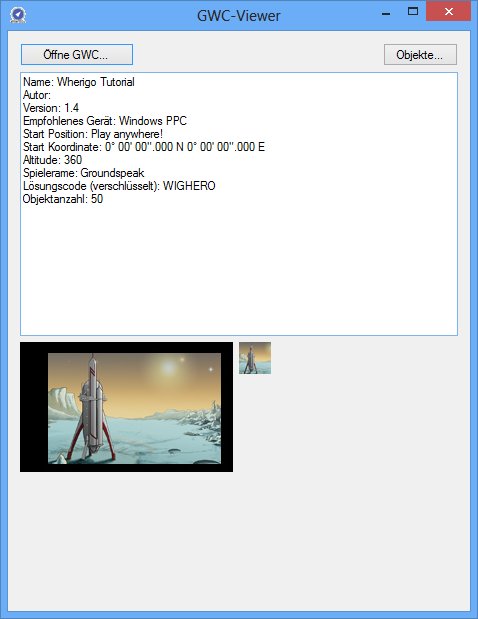
\includegraphics[width=0.5\textwidth]{screens/viewer_main}
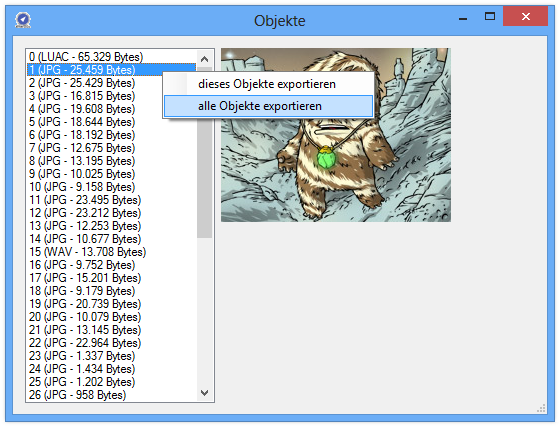
\includegraphics[width=0.5\textwidth]{screens/viewer_objects}

Der GWC-Viewer ist ein Hilfsmittel um zu sehen, welche Objekte (Sounds, Bilder) sich in dem Wherigo befinden. Diese kann man dann auch in den Ordner der Wherigo-Datei exportieren. Der LUA-Code (also das eigentliche Skript) ist compiliert und somit nicht lesbar, aber in einer sp"ateren Version des GWC-Viewers wird dieser Code auch dekompiliert sein.

\subsection{LuaTester}
Mit dem LuaTester wird es möglich sein, eigene Lua-Skripte auszuführen. Derzeit ist dieser noch nicht als Download verfügbar.
